% Set up page specifications and import packages
\documentclass[11pt]{amsart}
\usepackage[margin=.5in]{geometry}          
\usepackage{graphicx}
\usepackage{amsthm, amsmath, amssymb}
\usepackage{setspace}
\setlength{\parindent}{0em}
\usepackage{epsfig,bm,color}
\usepackage{mathtools}

\DeclarePairedDelimiter{\ceil}{\lceil}{\rceil}

% Define commonly used commands with a shortcut
\newcommand{\Zpx}{\mathbb{Z}_p[x]}
\newcommand{\Z}{\mathbb{Z}}
\newcommand{\Q}{\mathbb{Q}}
\newcommand{\C}{\mathbb{C}}
\newcommand{\R}{\mathbb{R}}
\newcommand{\e}{\epsilon}
\newcommand{\adj}{\rightarrow}
\newcommand{\tab}{\hspace*{.75cm}}
\newcommand{\setTo}{\leftarrow}
\newcommand{\ul}{\underline}
\newcommand{\kap}{\kappa}

% Define document tittle and author
\title{MA4710 Project 3}
\author{Daniel Henderson}

% Begin document and make tittle
\begin{document}
\maketitle

{\bf Introduction}\\

This week I explore adding categorical predictors and interaction terms into my linear model.\\

As explained in my first report, my data set comes from a survey that was posted on the /climbharder subredit.
In the survey, participants where asked to select an interval of how long they have been climbing.
The length of the interval was half a year, with the lower bound being 0 years, the upper bound being 15 years, and there was one additional category to select for those who have been climbing for more than 15 years.
Thus, in the raw dataset years climbing was a categorical predictor.
However, prior to this week I was using the lower bound of each interval to use years climbing as a numeric predictor in my model.
There where some linearity issues present when using years climbing as a numeric, which are addressed this week when we treat it as a categorical variable.\\

Since I had transformed years climbing in my data set to a numeric variable, I started this weeks investigation from scratch.
With the use of the na.omit function in R, I removed all observational units that where missing values in a numeric predictor field of the survey.
Next, there where various categorical predictors that where missing responses.
I eliminated any categorical variable that was left blank using the subset function in R.
Lastly, there where numerous survey participants who reported some of the numeric values in improper units.
I uncovered these observations in my diagnostic analysis and transformed such observational fields to units of centimeters and kilograms, where appropriate.
The resulting data set is found in 'FullData.csv', where Full refers to the dataset of survey participants who completed the questions as asked.
(there was no investigation to confirm that this elimination was done so without bias).
There are now $126$ observational units in this set\\

\newpage
{\bf Model Reduction}\\
We start this week's investigation by modeling hardest climbing grade as the response, with years climbing, hangboard frequency, sex, body mass index, and max pull-up reps as predictors. 
Initially, each predictor and all pairwise interactions between the predictors are included in the model.
As one could infer from my discussion of years climbing above, it was introduced into my model this week as a categorical predictor with 30 levels, where $0-0.5$ years experience as the control.
For various reasons, higher levels of years climbing produced many NA coefficients when it interacted pairwise with other predictors in my model.
I suspect this is due to a lack of observations in the uppers levels of years climbing. That is, not many people with $5+$ years of experience filled out the survey.
However the sport of climbing has grown drastically in the last 5 years. 
So our sample still may adequately reflect our population.
Nonetheless, to eliminate the NA coefficients I removed all interactions that included years climbing and I obtained the following model\\

\begin{center}
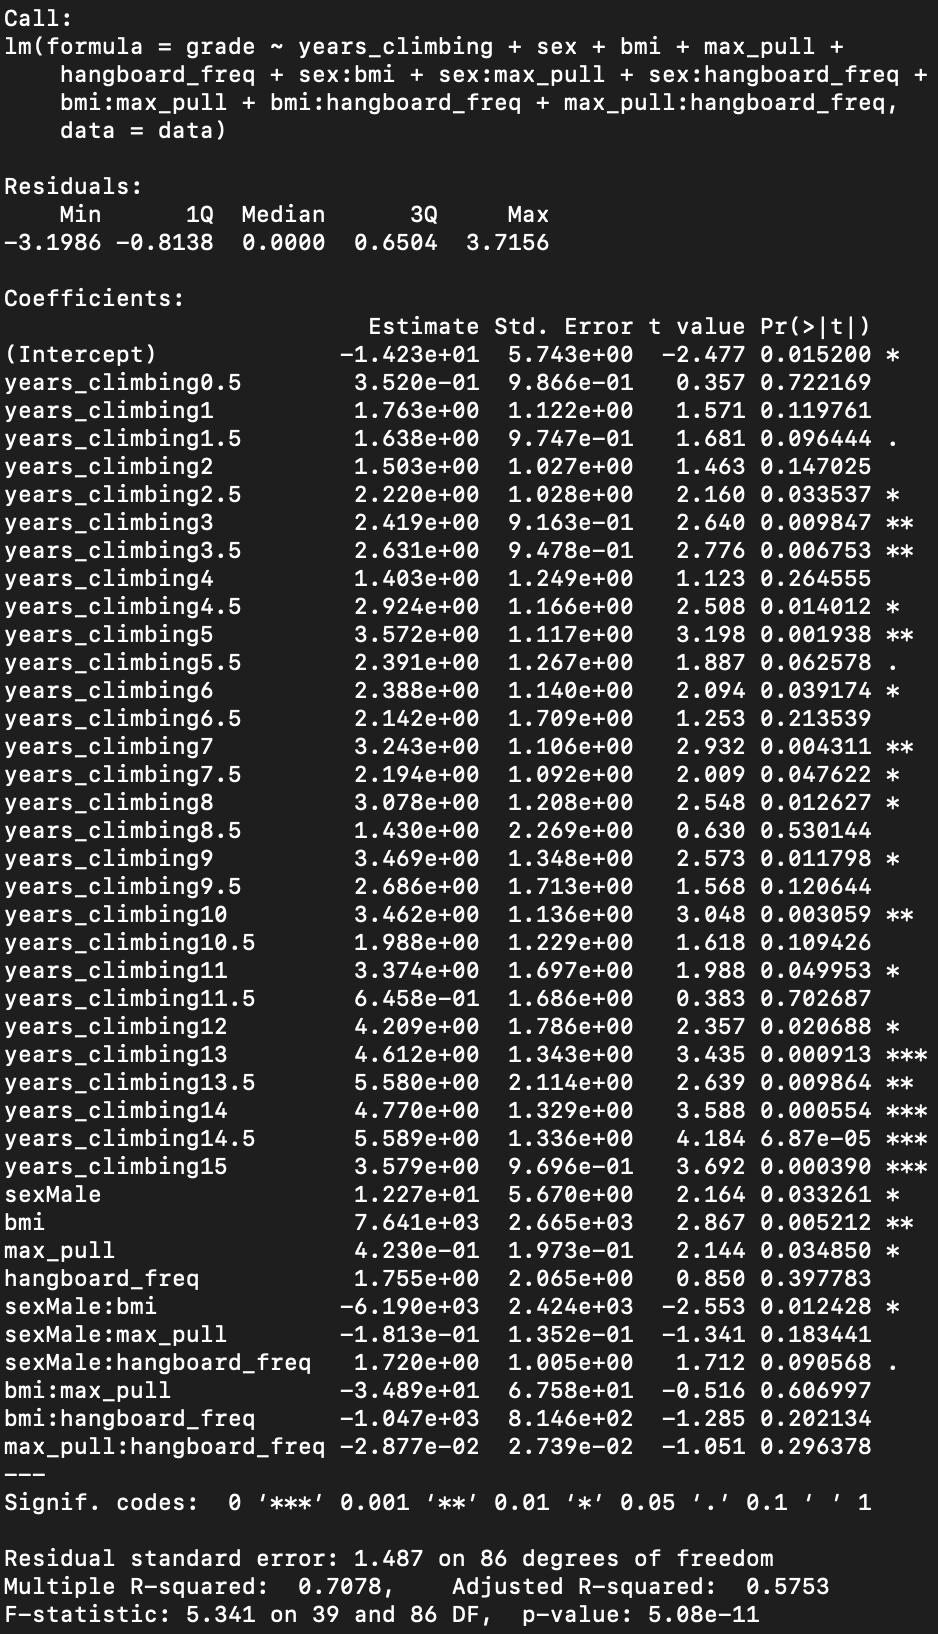
\includegraphics[width=0.5\textwidth]{mod1}
\end{center}
\vspace{0.15in}
Note that the lower bound of each level of years climbing is used to denote levels.
As you can see, the interaction term with the largest p-value is bmi:max\_pull.
We proceed by removing this term from the model

\newpage
{\bf Model Reduction Continued}\\
The new model is\\
\begin{center}
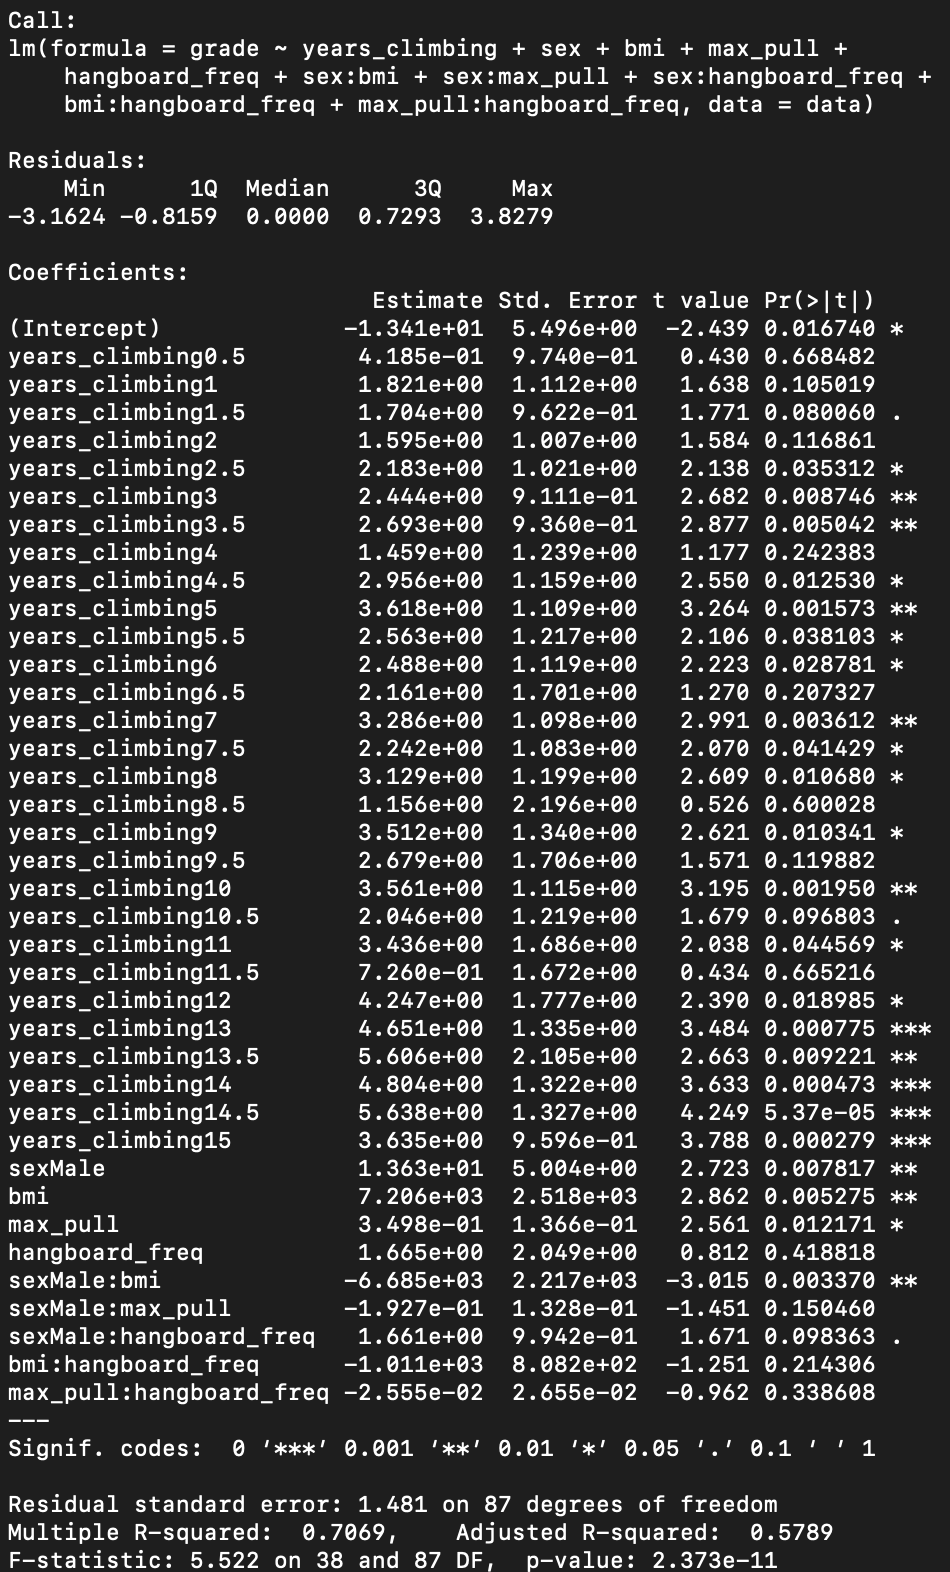
\includegraphics[width=0.65\textwidth]{mod2}
\end{center}
\vspace{0.15in}
As you can see, the interaction term with the largest p-value is max\_pull:hangboard\_freq.
We proceed by removing this term from the model

\newpage
{\bf Model Reduction Continued}\\
The new model is\\
\begin{center}
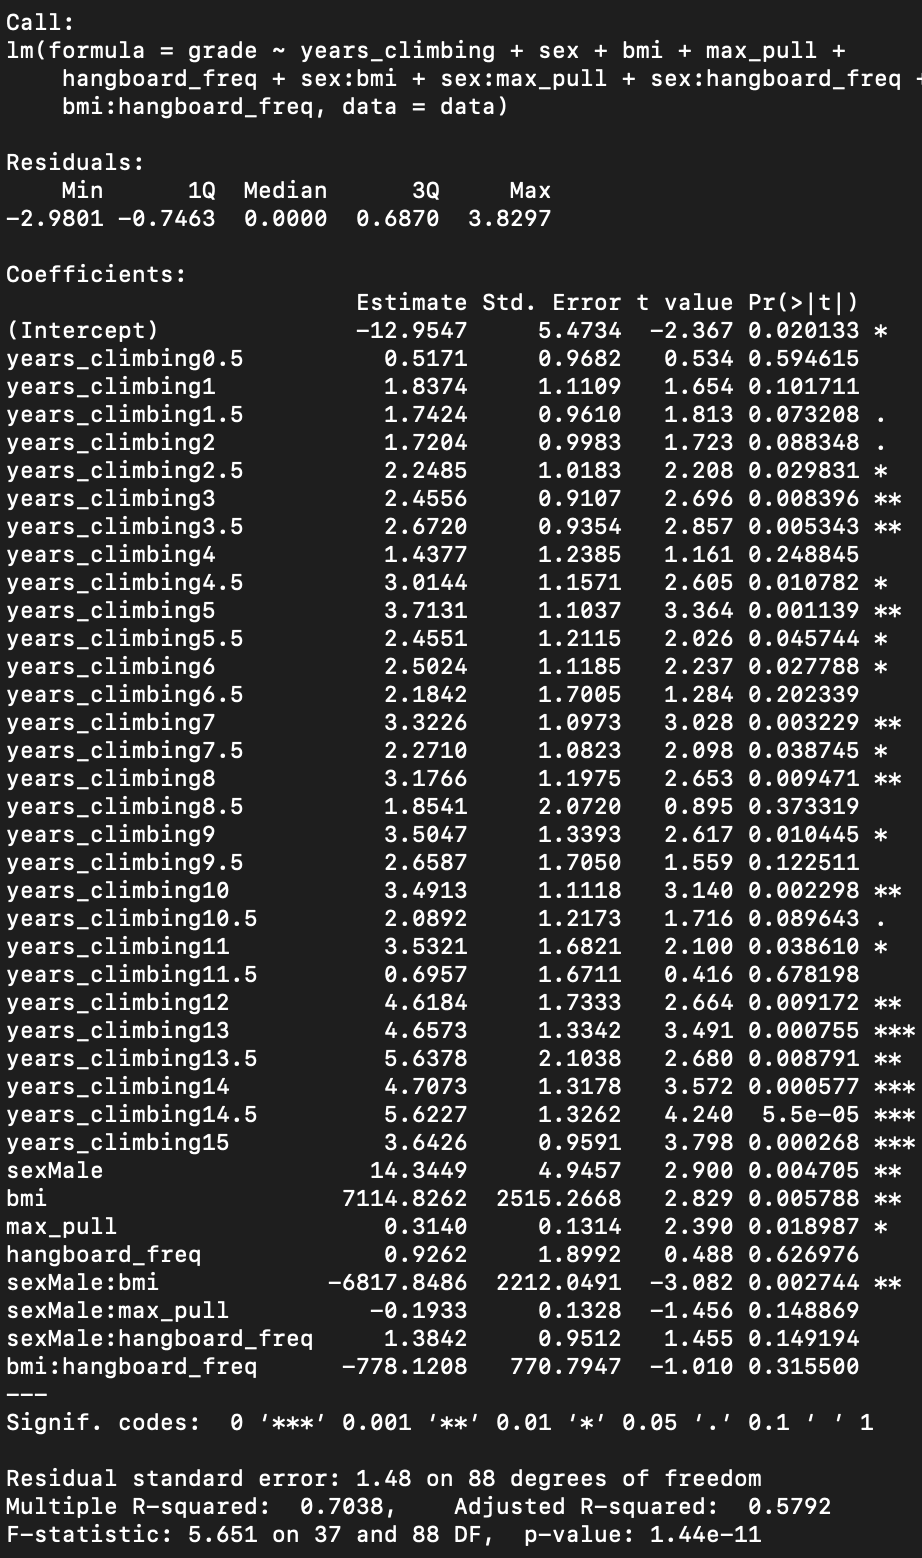
\includegraphics[width=0.65\textwidth]{mod3}
\end{center}
\vspace{0.15in}
As you can see, the interaction term with the largest p-value is bmi:hangboard\_freq.
We proceed by removing this term from the model

\newpage
{\bf Model Reduction Continued}\\
The new model is\\
\begin{center}
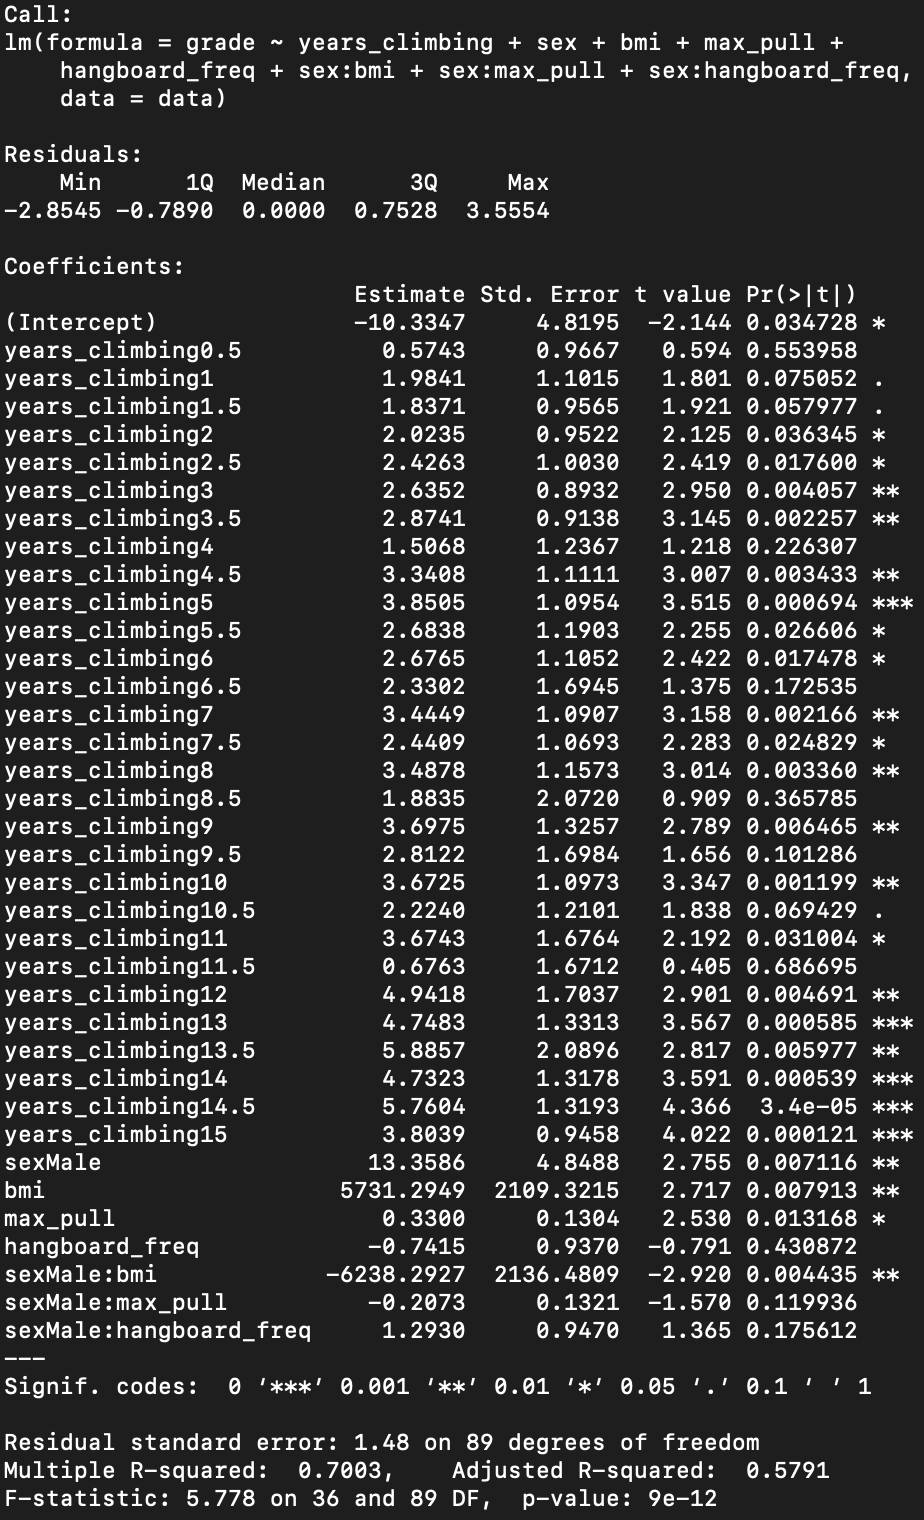
\includegraphics[width=0.65\textwidth]{mod4}
\end{center}
\vspace{0.15in}
As you can see, the interaction term with the largest p-value is sexMale:hangboard\_freq.
We proceed by removing this term from the model

\newpage
{\bf Model Reduction Continued}\\
The new model is\\
\begin{center}
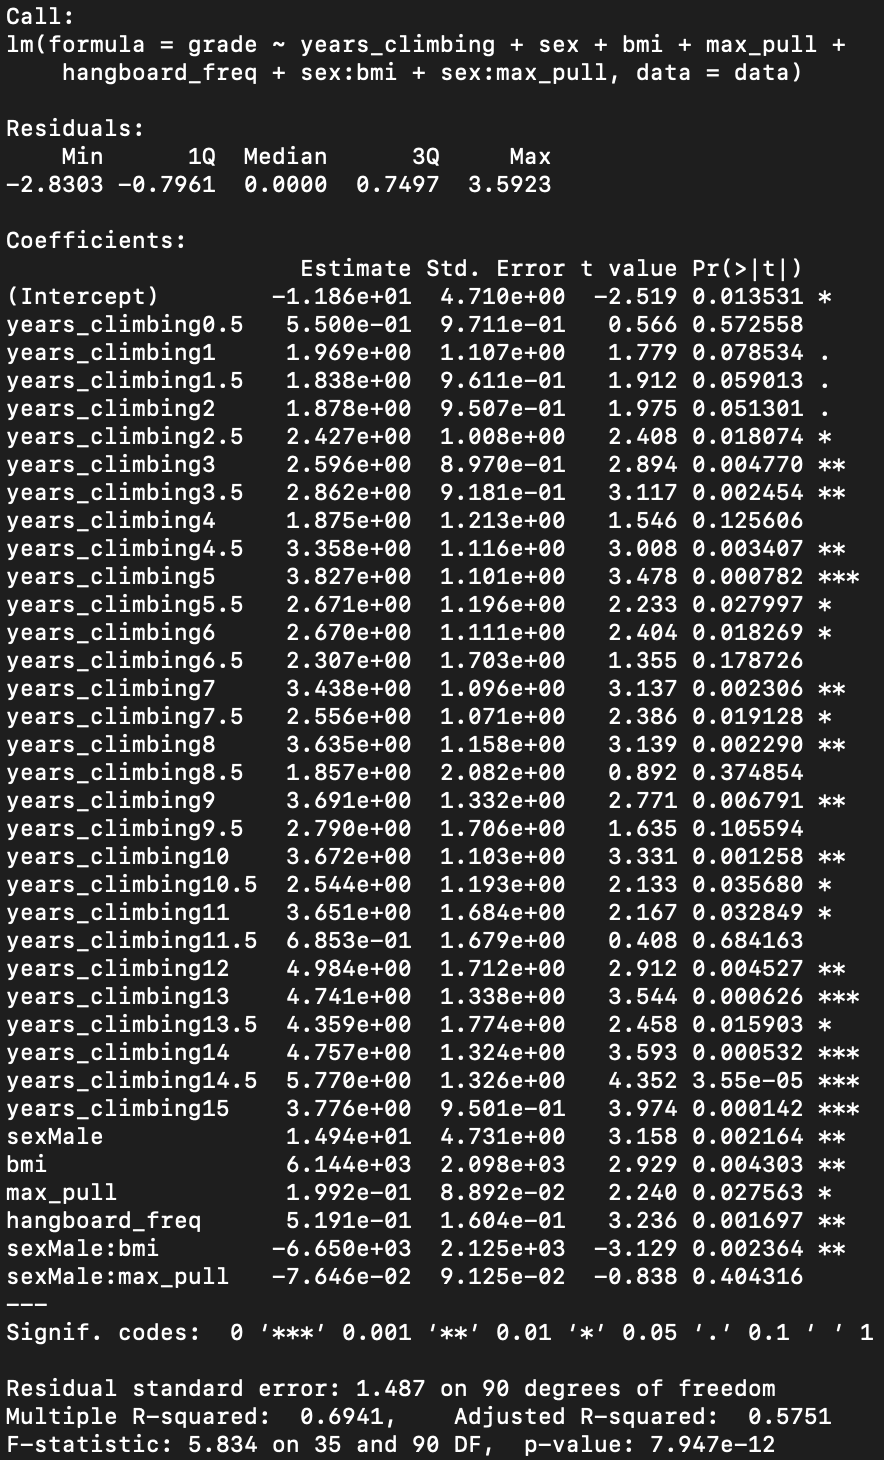
\includegraphics[width=0.65\textwidth]{mod5}
\end{center}
\vspace{0.15in}
As you can see, the interaction term with the largest p-value is sexMale:max\_pull.
We proceed by removing this term from the model

\newpage
{\bf Model Reduction Continued}\\
The new model is\
\begin{center}
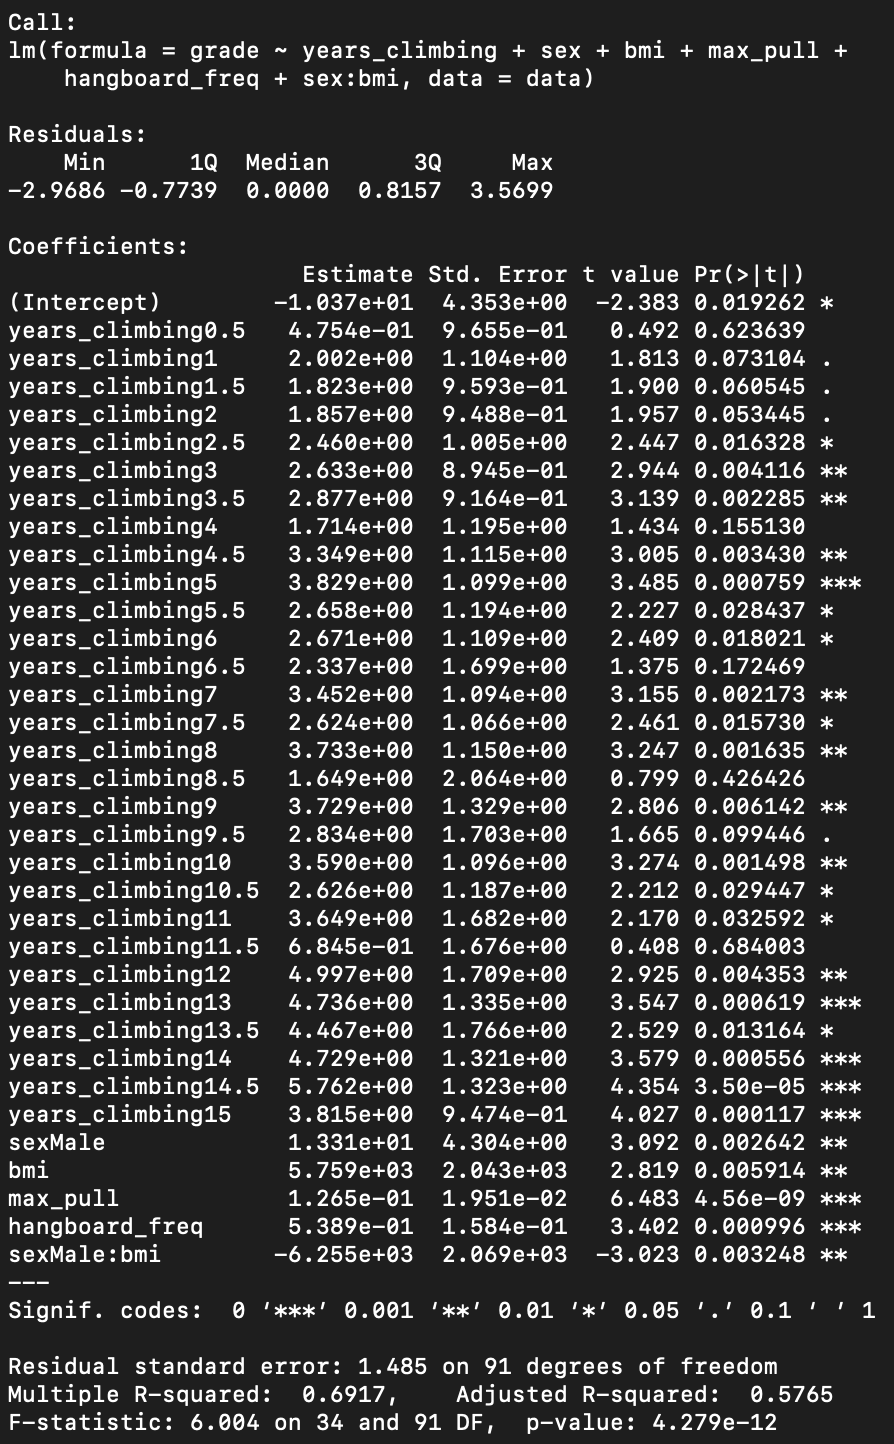
\includegraphics[width=0.65\textwidth]{mod6}
\end{center}
\vspace{0.15in}
This concludes our systematic reduction of interaction terms as specified by the assignment instructions.

 
 %%%%%%%%%%%%%%% DIAGNOSTICS %%%%%%%%%%%%%%%%%%
\newpage
{\bf Normality of Residuals}\\
The normal q-q plot, rather nicely, supports our assumption that the residuals are from a normally distributed population
\begin{center}
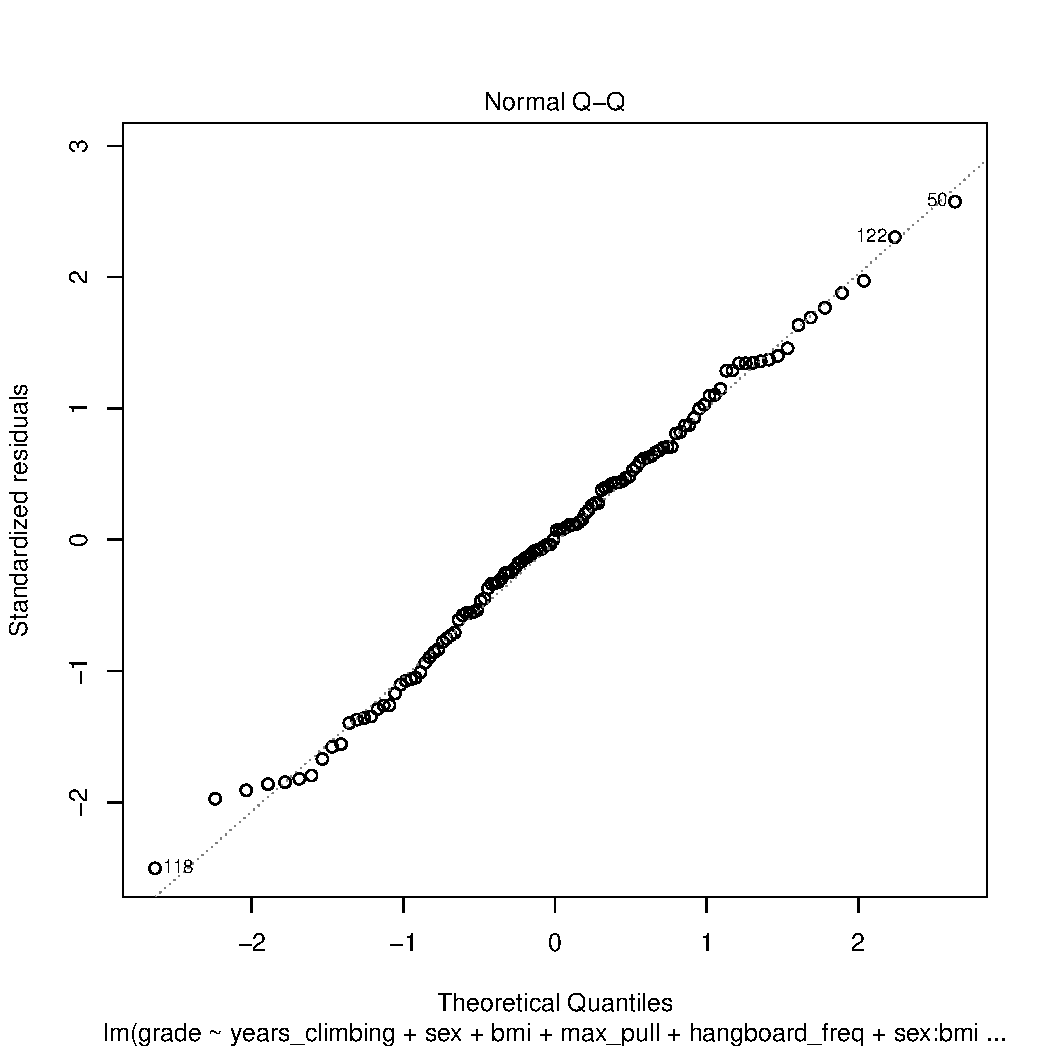
\includegraphics[width=0.55\textwidth]{1.pdf}
\end{center}
\vspace{0.15in}

This can also be seen from viewing the histogram\\
\begin{center}
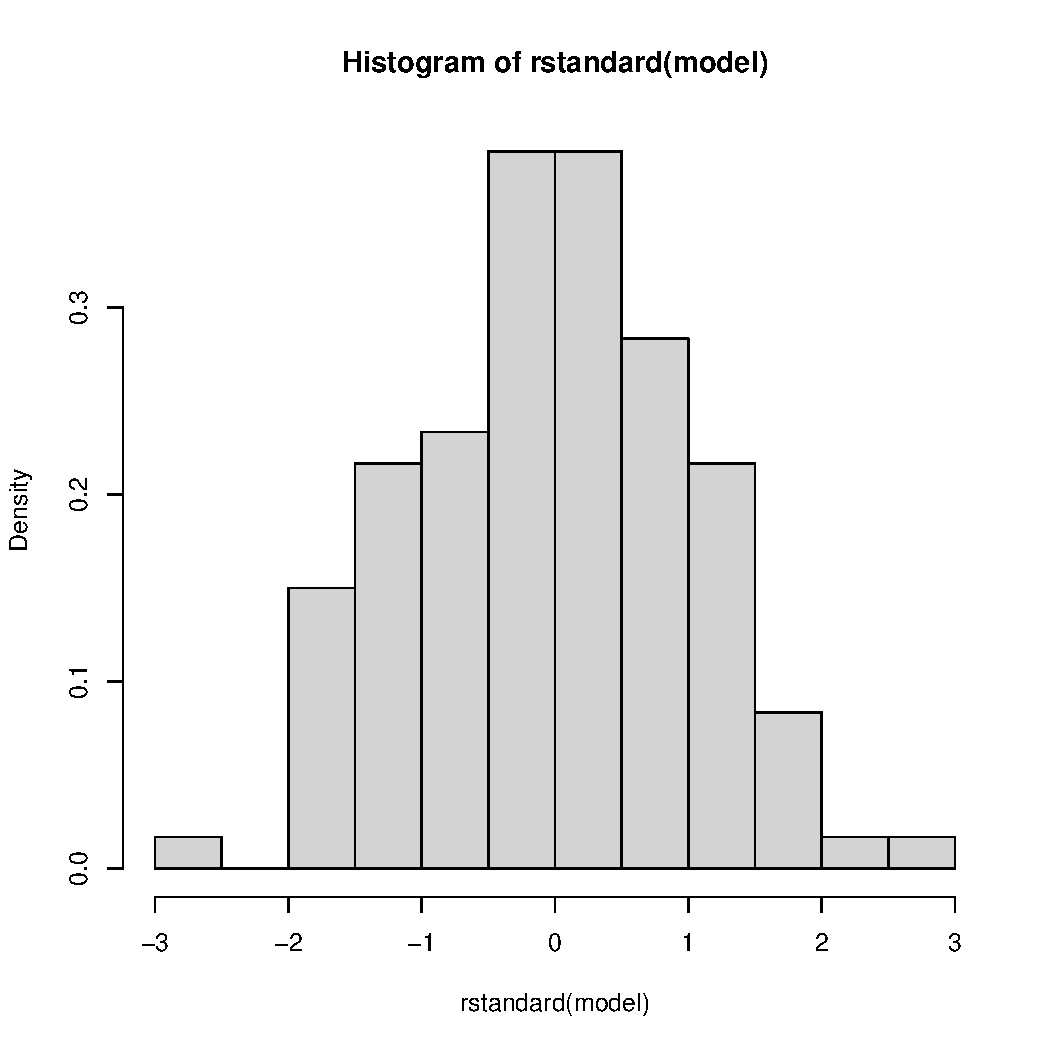
\includegraphics[width=0.55\textwidth]{2.pdf}
\end{center}

For further confirmation we find a p-value of 0.9083 in a Shapiro-Wilkes test.

\newpage
{\bf Linearity and Constant Variance of Residuals}\\
First observe the scale-location plot
\begin{center}
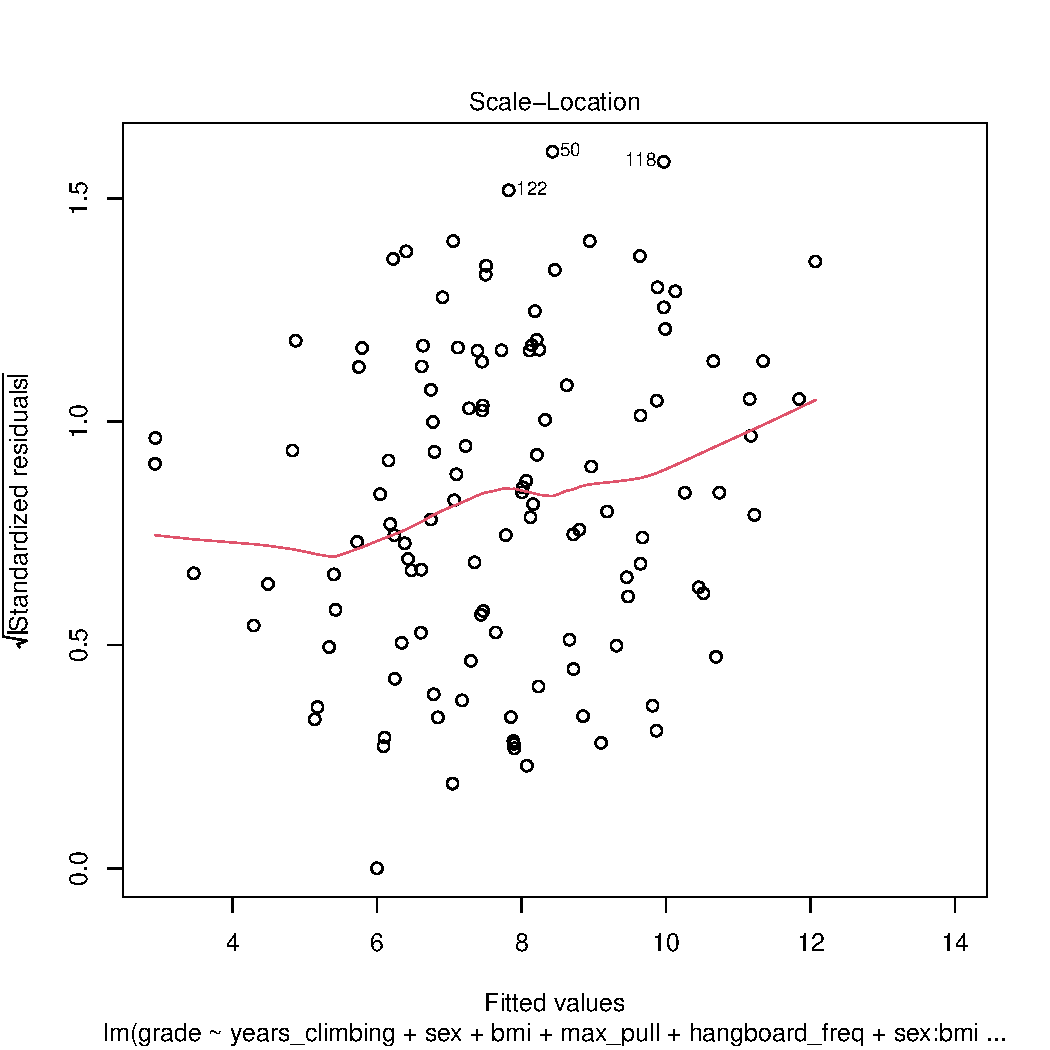
\includegraphics[width=0.7\textwidth]{4.pdf}
\end{center}
\vspace{0.15in}
There is nothing to concerning with this graph, as displayed by the lack of an obvious pattern.
It should be noted that the trace line increases slightly, which may imply that we are in violation of our constant variance assumption. But when viewing the non-standardized residuals verse fitted values graph that is shown on the next page, there is not an apparent funnel shape to our data. Therefore, we conclude that our homoscedasticity assumption holds. 


\newpage
{\bf Linearity and Constant Variance of Residuals Continued}\\
Next we asses our linearity assumption.\\
\begin{center}
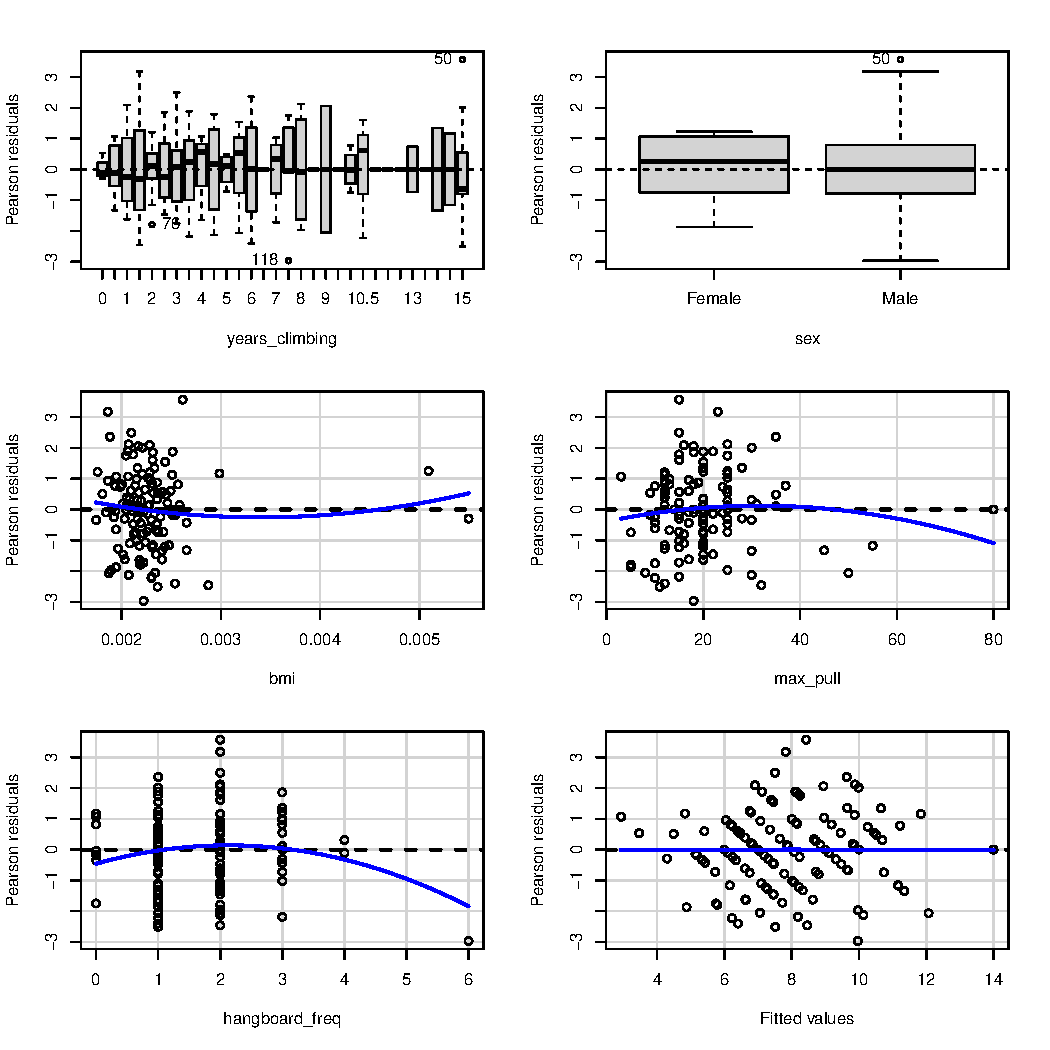
\includegraphics[width=0.6\textwidth]{3.pdf}\\\
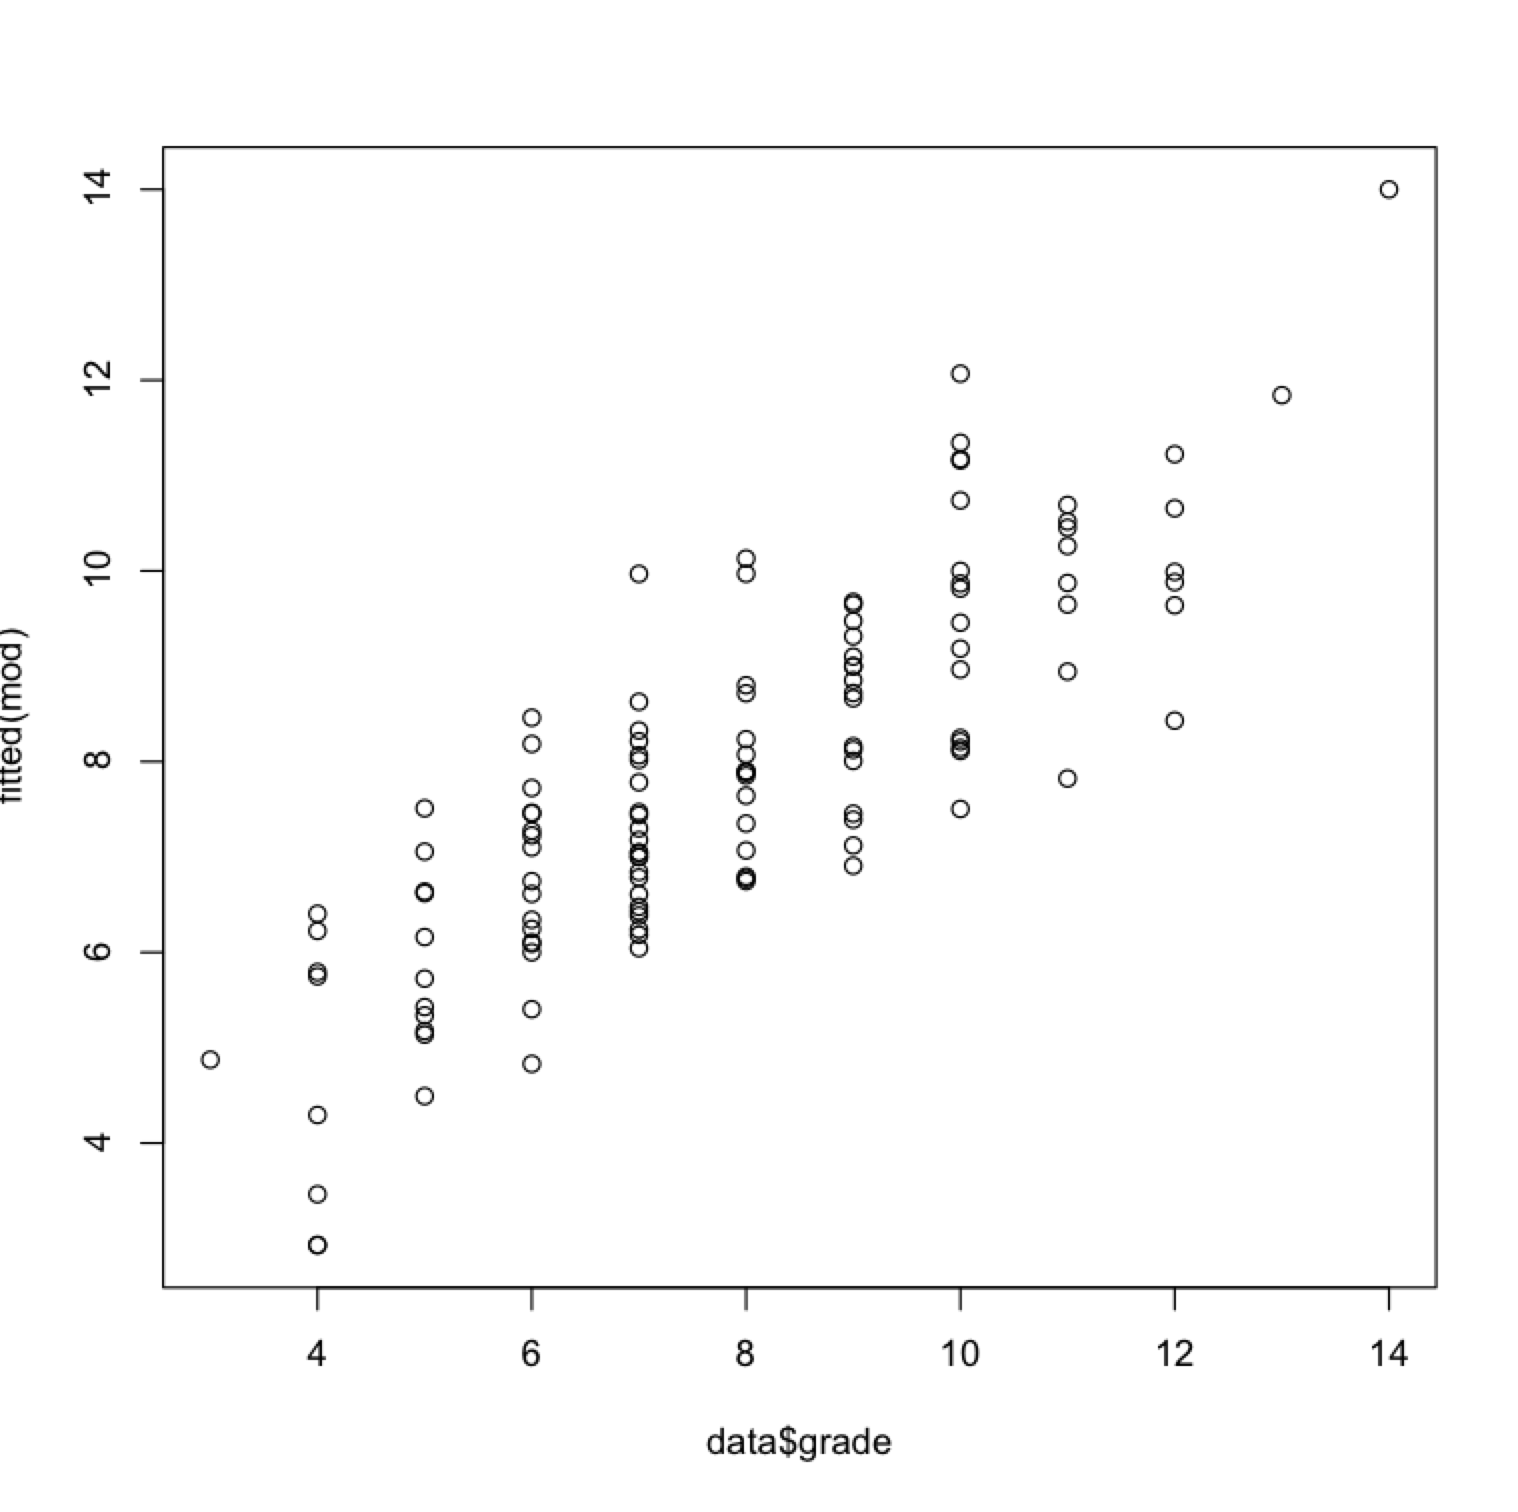
\includegraphics[width=0.6\textwidth]{lin}
\end{center}
\vspace{0.15in}
First, when looking at the residuals verse years climbing, the median observation for the residuals over the levels corresponding to climbers with less than $4$ years of experience tend to be negative. This may be an indication that the relationship between hardest grade and years climbing do not form a linear relationship.
I make this conclusion not only based upon the graph, but also because it makes sense when taking into account a basic learning theory model which would suggest that this factor be best modeled logarithmically.\\


Next it appears there may be an issue with the max pull predictor.
It may be overestimating the climbing grade for those who can manage to do $40$ or more pull ups. As numerically supported by the curvature test, which reports a p-value of $0.012$, which suggests nonlinearity. 
Next when looking at the weekly hangboard frequency as a predictor, there is an apparent outlier in this category that is influencing the quadratic line of fit.
The curvature test also supports a p-value of 0.05521, which may imply that there is more to be 
I would suspect this individual may be over training and it may be why he is climbing at a level far under the models mean predicted grade.\\

Lastly, the residuals verse fitted values do not indicate an apparent violation of our linearity assumption.
Nor does the plot of fitted values verse the observed values. 
However, our model may be improved by addressing some of the beforehand items.
So my conclusion is that our linear assumption is indeed suspect of violation.
Further discussion of how to deal with a potential linearity violation in our use of hangboard frequency occurs below.



\vspace{0.3in}
{\bf Influential Observations}\\
When examining out residuals verse leverage plot, there are no obvious influential observations.
Certainly some outliers, but there are no outliers with high leverage.\\

\begin{center}
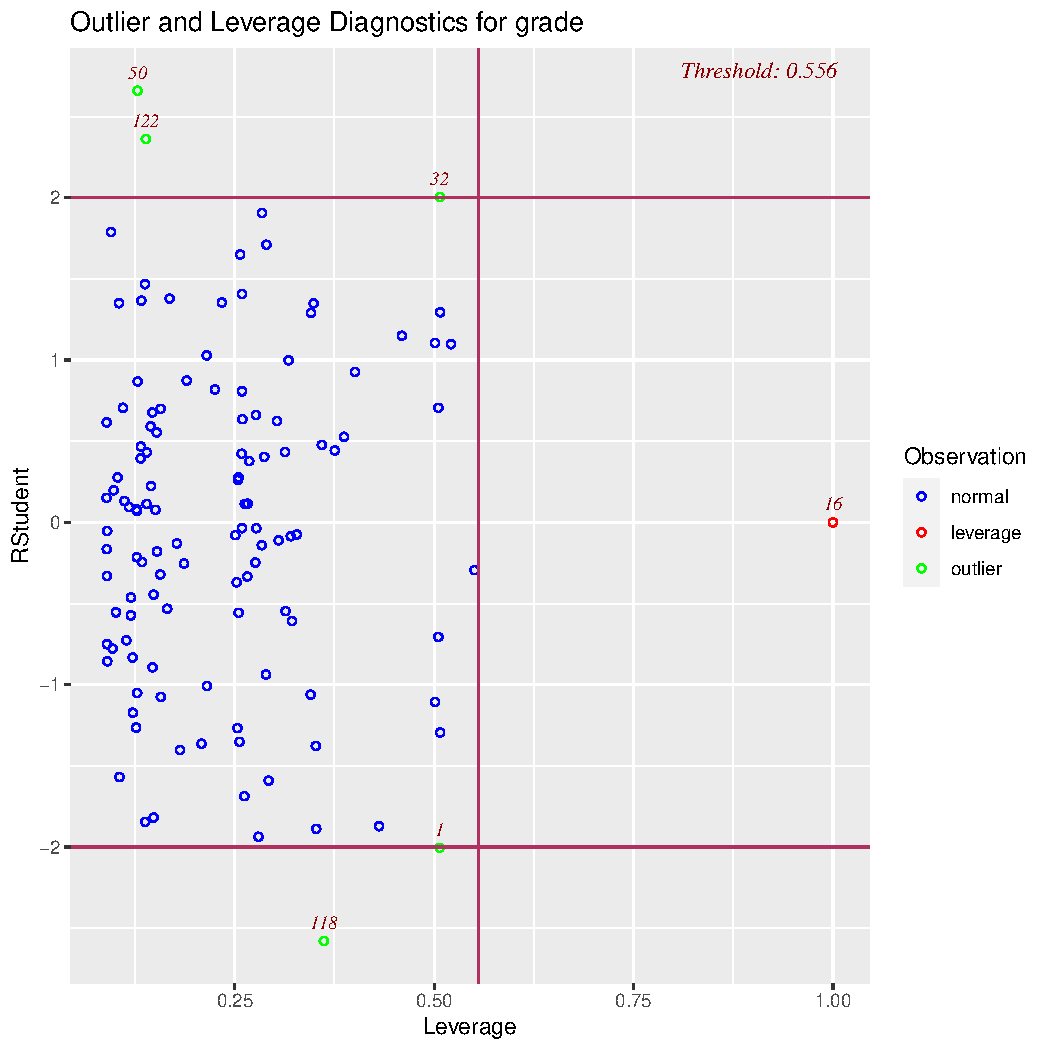
\includegraphics[width=0.6\textwidth]{5.pdf}
\end{center}
\vspace{0.15in}



On the next page we look at the DFFITS plot. We will use the rule that any DFFITS$_i > 2 \cdot \sqrt((p +1)/(n-p-1) = 1.271997$ should be labeled as influential. \\

\newpage
{\bf Influential Observations Continued}\\
\begin{center}
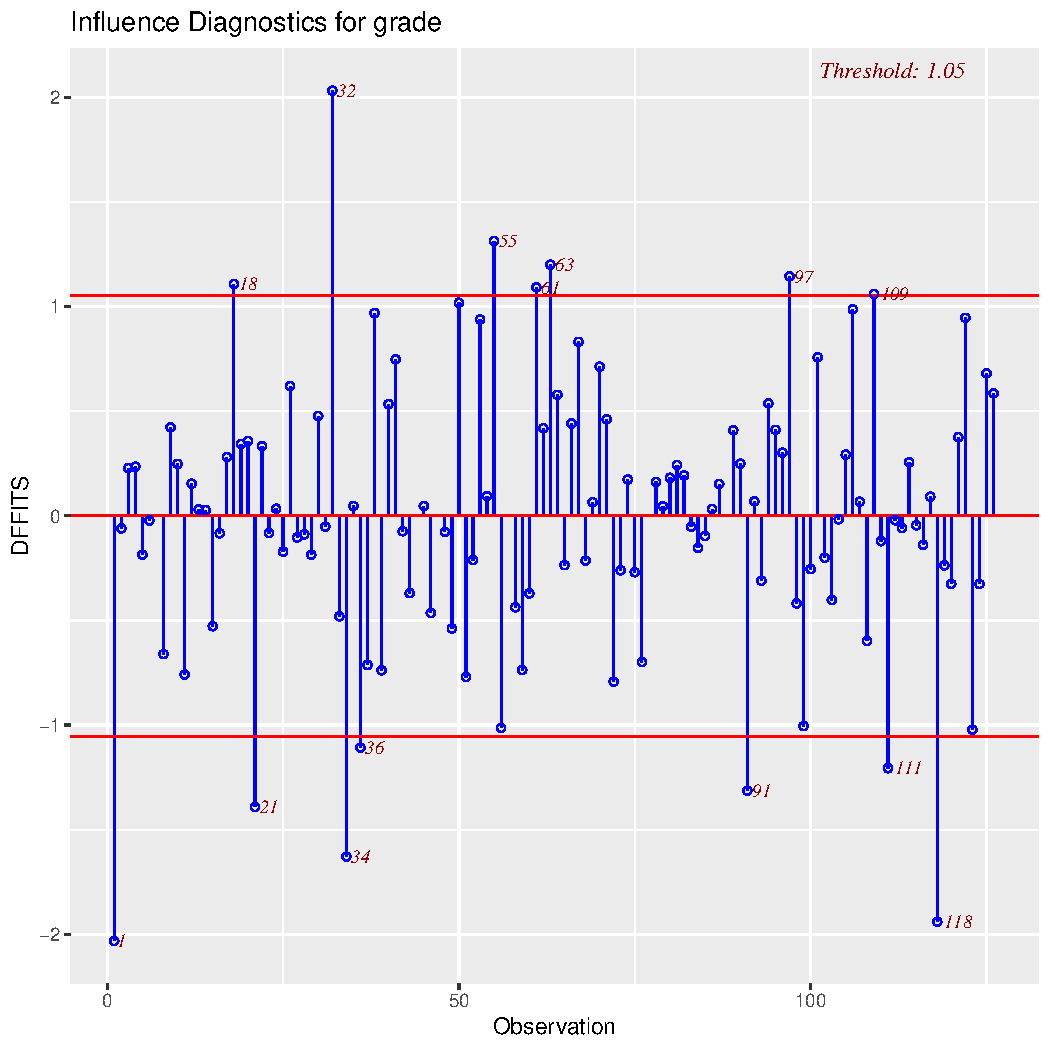
\includegraphics[width=0.6\textwidth]{15.pdf}
\end{center}
\vspace{0.15in}

There are a few influential points under this rule. Specifically observations $1, 21, 34, 91, 118$ and $32$.

Due to all the categories in years climbing the DFBETA index plots show an enormous amount of information and not much of it is meaningful. There was one observation that was deemed influential by the threshold line created from the dfbetaPlots in the car package. Specifically, it was observation 97 that influenced the weekly hangboard frequency coefficient drastically and this was the same outlier that was identified in our linearity discussion. However, the observation also happened to be a very elite climber and there where very few of those so consequently it impacted the hangboard frequency coefficient.\\

This is a symptom in of my underlying model. In my opinion there are few possible solutions:\\
\tab (1) Blame the messy data. Ideally, we could collect a sample that would contain more elite climbers.\\
\tab (2) Model weekly hangboard frequency as a categorical predictor instead of a numerical variable.\\
\tab (3) Remove the observation.\\

The first option is the easy way out. Then for the second, when replacing it as a categorical factor in our model and performing an F-test yields a p-value of $0.13$ (adjusted $R^2$ decreases to $0.597$). These results imply that our current treatment of hang board frequency should remain as is and further investigation into a suitable transformation should be performed (either on the numeric or categorical data).
As for removal, there are no obvious inaccuracy's in observation $97$. One could even argue that due to observation $97$'s level of climbing, his responses are likely the most accurate. 
If the goal of the model is to be used for predicting and training purposes then the best solution is to remove the observation.
However, if we are trying to make a statistical inference on the population it is likely best to leave as is.
Though that opens an entirely new discussion as to what our population is, if it is of all climbers then the chances observing a climber of this level in our sample size is quite small. 
Hence, an argument still may be made for removal. \\

The model will remain as is.

\newpage
{\bf Interpretation of Interaction Terms}\\
The only interaction term in my model is between the numeric bmi and the categorical sex.
However, we also include sex and bmi independently so it is a "different slopes, different intercepts" model.
The variable bmi was calculated from the reported height and weight values.
R decided to have Female as the control for the sex dummy term in the model.
The coefficient on bmi refers to the slope for female climbers.
Then the interaction term between bmi and sex effectively reduces the bmi coefficient (by a very small amount) when a male climber is being inputed into the model
But the presence of the male climber changes the intercept of the model.
Apart from this, there really isn't a meaningful way to describe the coefficient between the interaction of male and female.
\vspace{.3in}

{\bf Linear Hypothesis Test of Years Climbing}\\
Given so many levels to the categorical variable of years climbing, our model may benefit from collapsing some of the categories. This may also eliminate all of the NA coefficients that appeared when I tried to make this variable interact with others in my model.
Which may allow us to have years climbing interact with other terms and lead to a much better model.
This will be investigated in the next submission.
Since the majority of the NA's appeared in the levels of experience greater than 5.5 years, I did a crude test to see if collapsing everyone who has been climbing for 5.5-15+ years into one category would suffice. The p-value with this test is $0.2686$, so we will keep the original model for now.


\end{document}